%!TEX root = ../../thesis.tex

NIR spectroscopy...

Spectrograph design stuff


\section{NIR spectroscopy}
To perform spectroscopy requires an instrument called a spectrograph. The purpose of which is to take the incoming star light and disperse it so that the different wavelength components separate. A simple example of this is the splitting of white light into a rainbow when passed through a prism.

All spectrographs are comprised of a few key components.
The first part is the front end optics responsible for collecting the light and getting it to the spectrograph, such as a telescope, entrance slit or fibre.
The second part component dispersive elements inside the spectrograph, such as a prism or grating used to separate the wavelength components.
The final part is the detector or camera, used to record the resulting spectrum.

The design of spectrographs is highly dependant on the wavelength range observed. For instance {CCD} cameras (based on silicon) are readily used in the optical but silicon is a poor detector at \nir{} wavelengths.
Instead \nir{} spectrographs need to use CMOS detectors which are composed of different materials that are sensitive to different wavelengths.
{CRIRES} detectors specifically are made of \ce{InSb} (Indium antimonide) to perform spectroscopy between 1--5\um{}~\cite{dorn_crires_2004}.
Other considerations are needed such as the composition of the optical components as well as any anti-reflection coatings used, all of which have different wavelength characteristics that need to be matched.

\todo{I don't know where I am going with this section.}




Observing in the \nir{} is specifically desirable for the cooler sub-stellar and giant planet companions as their thermal emission is stronger in the infrared compared to the optical.
This improves the contrast ratio between the host star and companion, providing favourable conditions for their detection and spectral separation.


\textbf{Goal for 29th October 2018 - Details about spectrographs complete }

\subsection{CRIRES}
CRIES (Cryogenic Infrared Echelle Spectrograph) is an ESO IR spectrogrpah that was mounted on the Unit Telescope (UT1, Autu) of the European Southern Observatory Very Large Telescope (VLT)~\citep{kaeufl 2004 } from XXX \textbf{p 79} - though July 2014\footnote{Note this PhD research began in October 2014.}.

The main optical elements consist of a prism pre-disperser and a 31.6\,lines/mm echelle grating. The instrument provides resolutions up to 100\,000 when used with a 0.2\arcsec slit.\footnote{The rule of thumb resolution is R = 100\000\times\frac{{slit width}}{0.2\arcsec}}. The wavelength range is 960--5200\nm with an instantaneous wavelength coverage of \(\sim \lamda/50\). The spectra are imaged on a detector mosaic, consisting of four Aladdin III detectors (\(4096 \times 512\) pixel) in a row, with a gap of \(\sim 250\) pixels between each chip. Adaptive optics (MACAO - Multi-Applications Curvature Adaptive optics) can be used to optimize the signal-to-noise ratio and the spatial resolution. \Cref{fig:criresschematic} displays the schematic representation of the CRIRES optical layout.

CRIES lead the way for high-resolution spectrograph in the IR with a resolution higher than any of its predecessors, and unique capabilities, like AO. As with any new instrument there were several problems that affected CRIRES during its Science operations. For instance there were several mechanical issues with the slit; the slit edges were not parallel and there were issues with precise and reproducible positioning. Other issues such as Detector glow, the odd even effect and the wavelength calibration are corrected detailed in \cref{subsubsec:darkcurrent,subsec:flat-field,subsec:wavecalib}.


\begin{figure}
    \centering
    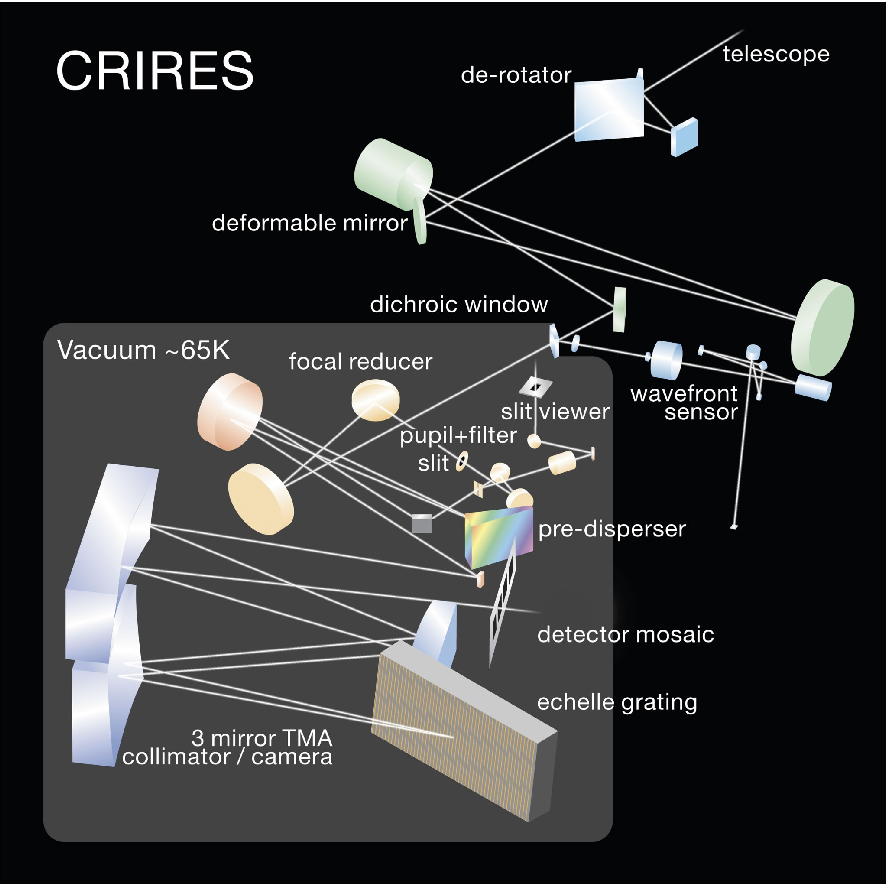
\includegraphics[width=0.7\linewidth]{figures/advanced_material/CRIRES_schematic}
    \caption{CRIRES layout schematic, from the CRIRES manual v93.}
    \label{fig:criresschematic}
\end{figure}

